\documentclass[xcolor=table]{beamer}
\usepackage[table,xcdraw]{xcolor}
\usepackage[utf8]{inputenc}
\usepackage{epigraph}
\usepackage{graphicx}
\usepackage[left=25mm,right=25mm,top=2cm,bottom=2cm]{geometry}
\usepackage{indentfirst}
\usepackage{hyperref}
\usepackage{amsmath}
\usepackage{xcolor}
\usepackage{float}
\usepackage{wrapfig}
\usepackage{subfig}
\usepackage{derivative}
\usepackage[table,xcdraw]{xcolor}
\usepackage[english, russian]{babel}
\usepackage{setspace}
\usepackage{hyperref}
\usepackage{movie15}
\usepackage{animate}


\usetheme{Madrid}
\usecolortheme{default}

%------------------------------------------------------------
%This block of code defines the information to appear in the
%Title page
\title[Получение и измерение Вакуума] %optional
{Получение и измерение Вакуума}

%\subtitle{Начало}

\author[Аношин, Шашков] 
{М.~Аношин\inst{1} \and Д. ~Шашков\inst{1}}

\date[11.02.2023] 
{МФТИ, Февраль 2023}

\begin{document}
\frame{\titlepage}

\section{Цель работы}
\begin{frame}\frametitle{Цель работы}
    \large \textbf{Цель работы - Получение и измерение параметров высокого вакуума}  
    
    \large{\\ В работе используются: Вакуумная установка с манометрами: масляным, термопарным, ионизационным.}\\
    \begin{itemize}
        \large \normalsize{}
    \end{itemize}
\end{frame}


\begin{frame}\frametitle{Установка}
    \begin{figure}
        \centering
        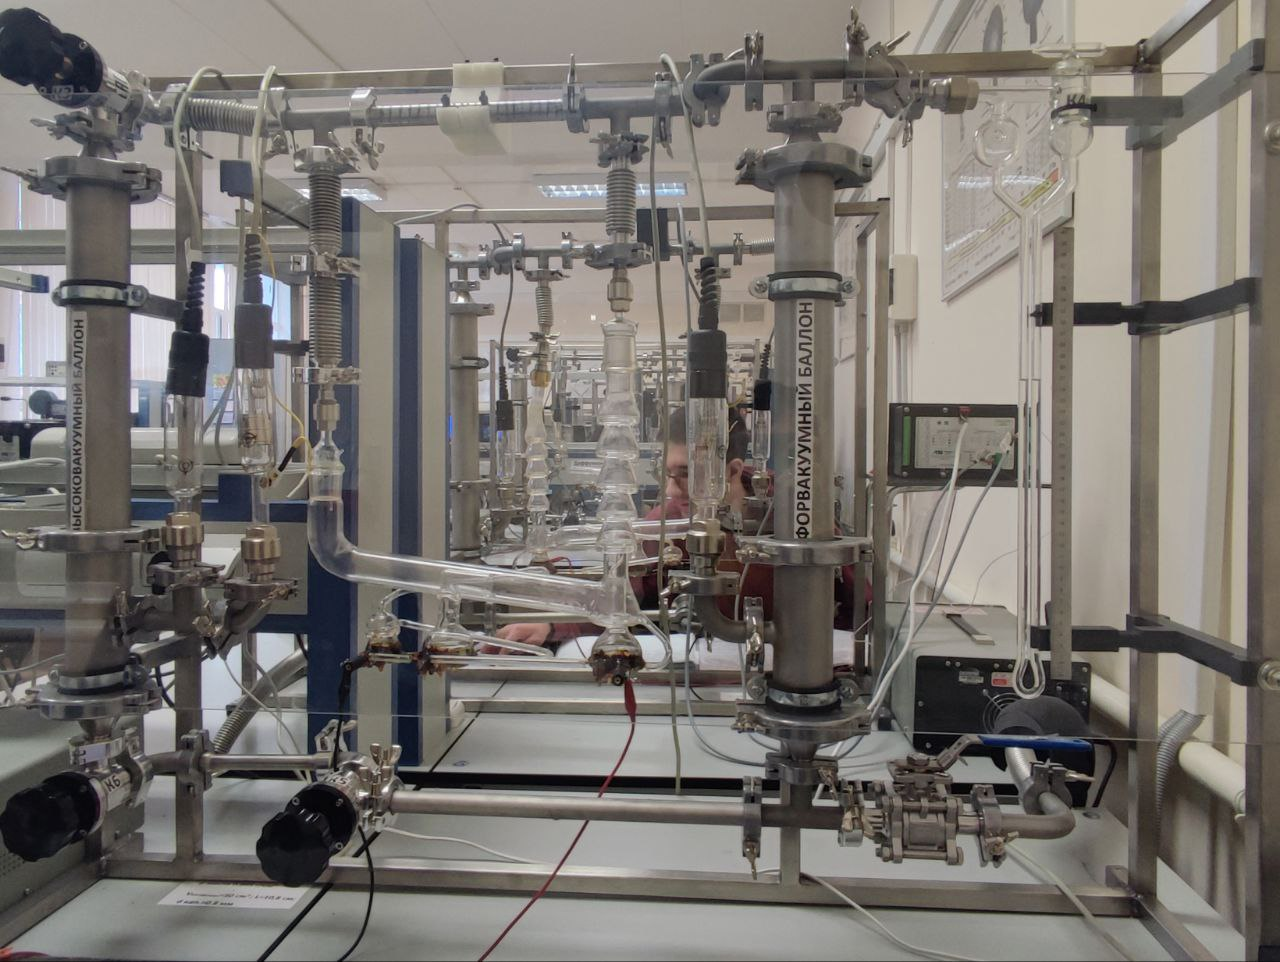
\includegraphics[scale=0.2]{images/full.jpg}
        \caption{1. Полная фотография установки}
        \label{fig:my_label}
    \end{figure}
\end{frame}


\begin{frame}\frametitle{Ход работы: определение объёмов}
    Изначально все краны открыты, в установке находится атмосферный воздух. Далее закрываются краны \textbf{5} и \textbf{6} и включается форвакуумный насос, объём запертого в перемычке между ними воздуха \(V_1 = 50 \text{ см}^3\)
    \begin{figure}
        \centering
        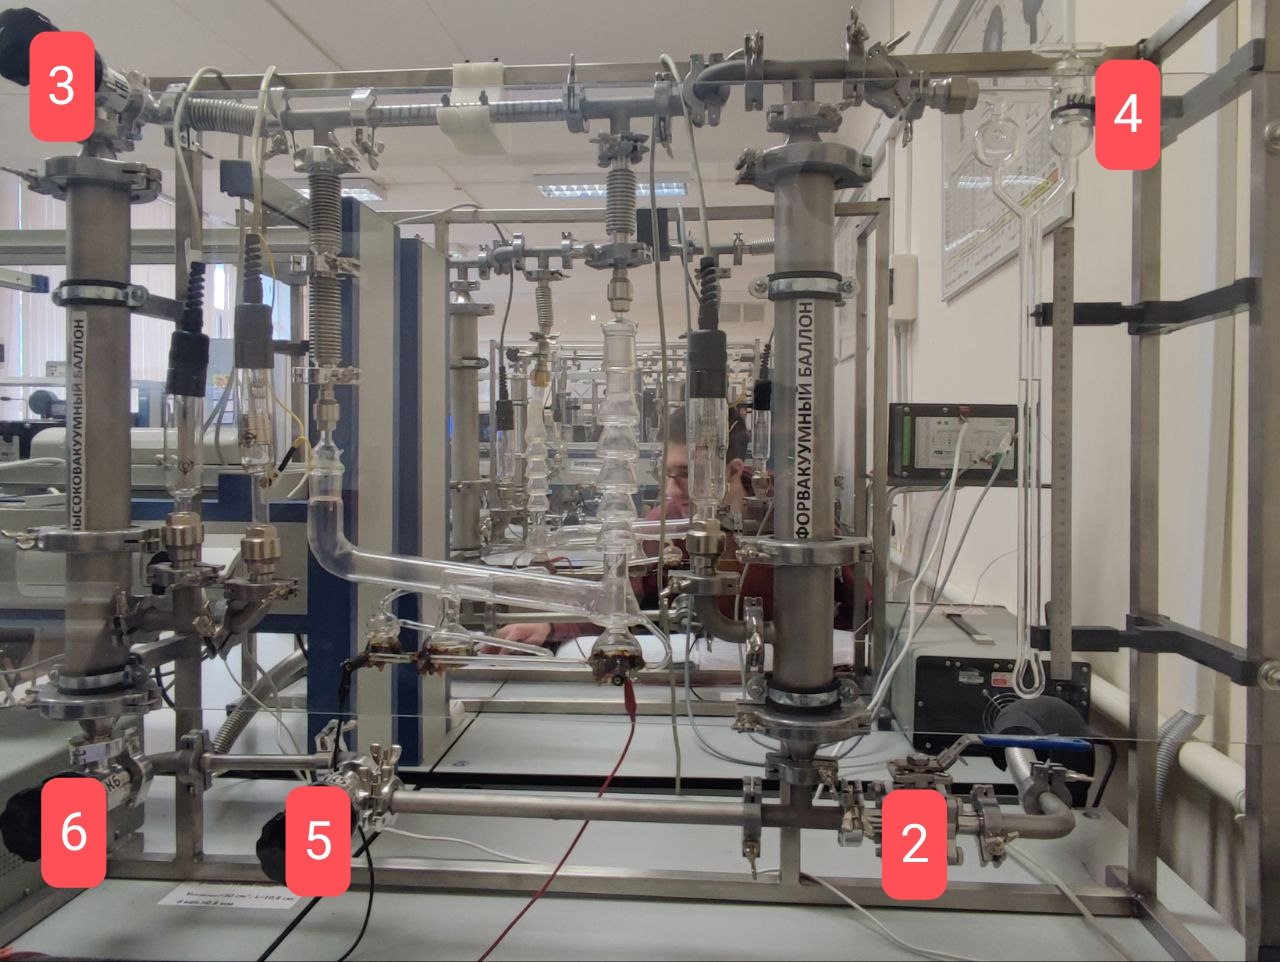
\includegraphics[scale=0.19]{images/valve.jpg}
    \end{figure}
\end{frame}


\begin{frame}{Ход работы: определение объёмов}
    По достижении \(p_{c0} \approx 10^{-2}\) мм.рт.столба закрываем \textbf{2} и \textbf{4} краны, форвакуумный насос работает. Манометр уже готов к работе, в его правом колене вакуум. 
    \begin{figure}
        \centering
        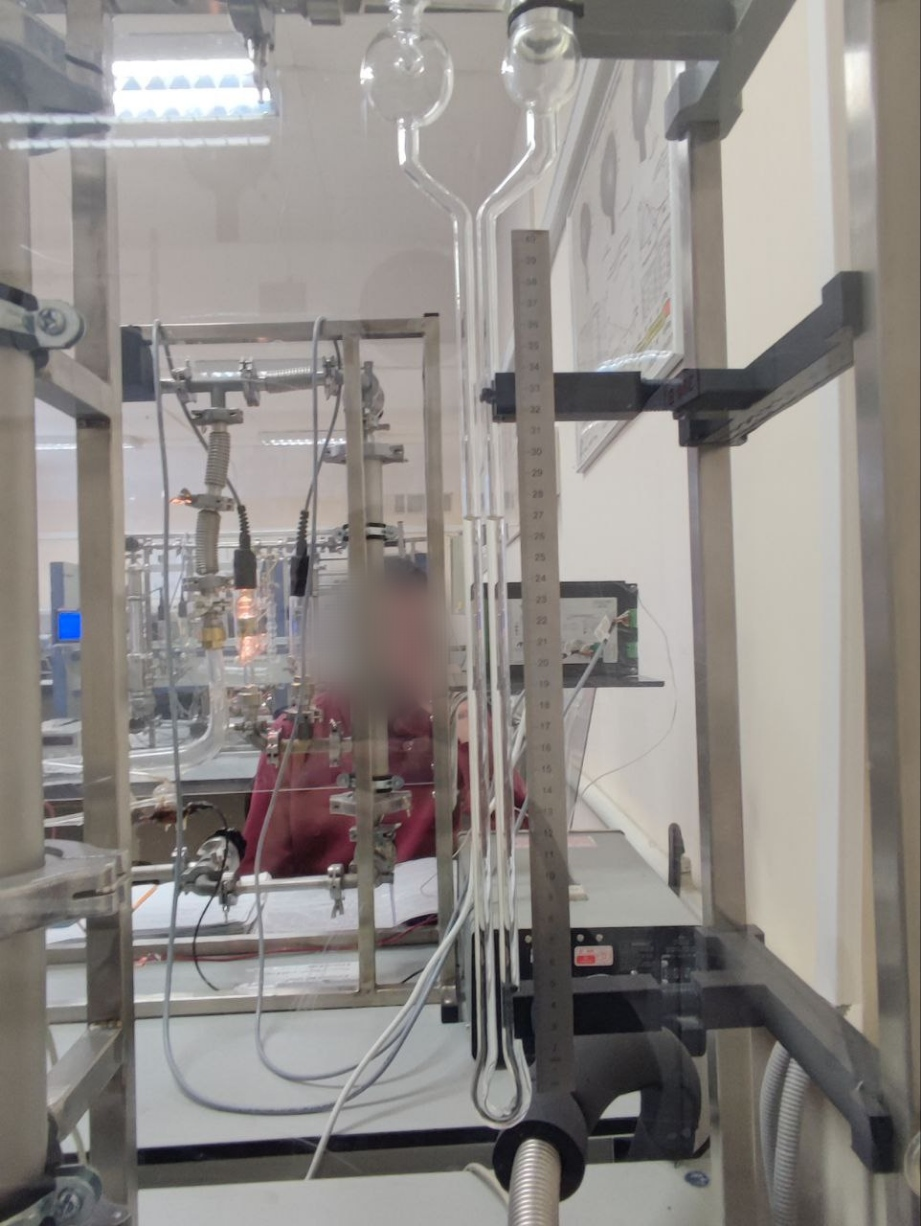
\includegraphics[scale=0.15]{images/oil_manometer.jpg}
    \end{figure}
\end{frame}


\begin{frame}{Ход работы: определение объёмов}
Далее закрывается \textbf{3} кран, отделяющий форвакуумную часть от высоковакуумного баллона. Масляный манометр показывает высоты (см.масл.столб)
\begin{table}[h!]
\begin{tabular}{|c |c|}
\hline
h_{up} & h_{down} \\
\hline
39.9      & 12.9  \\    
\hline
\end{tabular}
\end{table}
Что дает давление: 
$p_1= 27 \text{ см.масл.столба} = \text{17.36 мм.рт.столба} $

Откуда объем форвакуумной части (\(T = T_{room}\)) \(V_f=V_0\frac{p_0}{p_1}=3.1 \text{ л}\)

\end{frame}


\begin{frame}{Ход работы: определение объёмов}
    Далее открывается высоковакуумный баллон, и манометр показывает \\ \begin{table}[h!]
\begin{tabular}{|c |c |}
\hline
h_{up} & h_{down} \\
\hline
35.3      & 18.3   \\
\hline
\end{tabular}
\end{table}
Откуда давление в системе: 
$p_2=\rho g (h_1-h_2) = 17 \text{см.масл.столб}$

И объем баллона \(V_h=V_f(\frac{p1}{p2}-1)= 1.82 \text{ л}\)
\end{frame}


\begin{frame}{Ход работы: создание высокого вакуума}
    После измерения объёмов открываем \textbf{все} краны, откачиваем воздухю \\
    Проводим измерение давления в высоковакуумной и форвакуумной частях при помощи термопарных манометров.
    \begin{figure}[h]
        \centering
        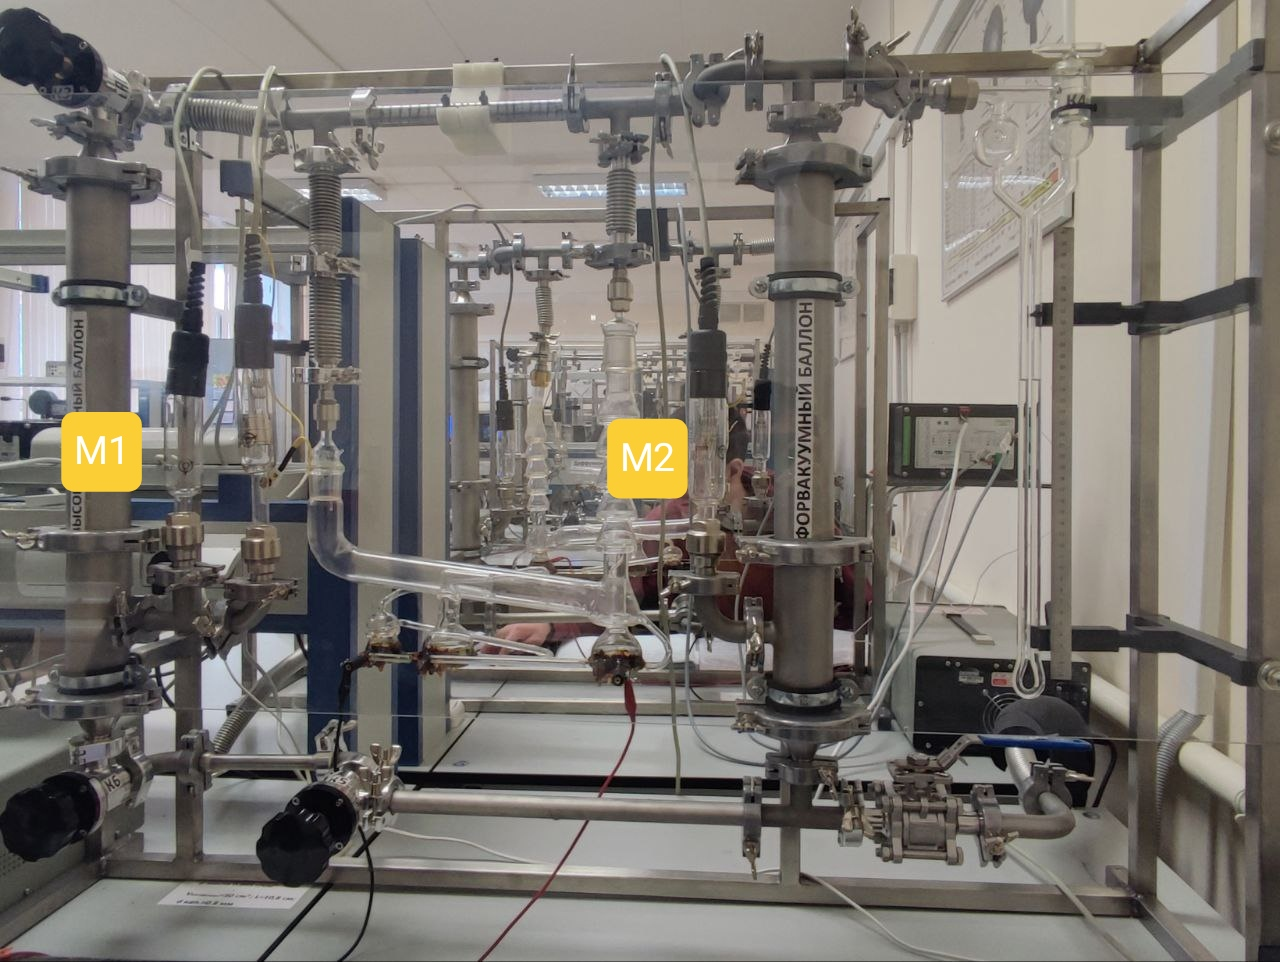
\includegraphics[scale = 0.15]{images/therm.jpg}
    \end{figure}
\end{frame}


\begin{frame}{Ход работы: создание высокого вакуума}
    При достижении давления \(p_{c0}\) закрывается кран \textbf{6},  высоковакуумный баллон остаеться связаным с форвакуумной частью только включенным масляным насосом.
    \begin{figure}[h]
        \centering
        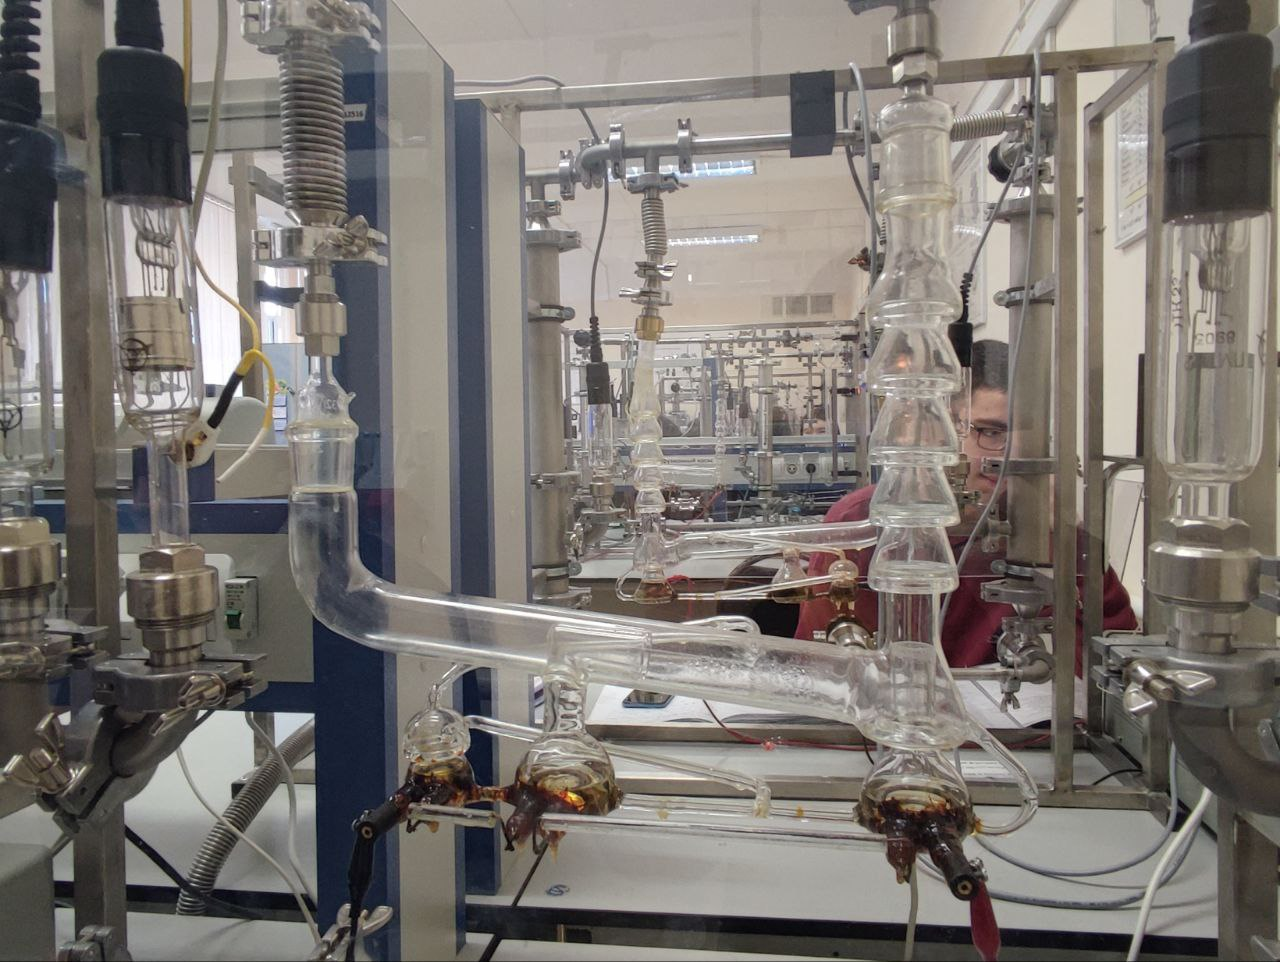
\includegraphics[scale = 0.15]{images/oil_valve.jpg}
    \end{figure}
\end{frame}



\begin{frame}{Ход работы: создание высокого вакуума}
    Когда давление в высоковакуумном баллоне становится ниже \(p_{c1}=1.2 \cdot 10^{-4} \text{ мм.рт.столба }\)
    происходит инициация ионизационного манометра. Можно приступать к измерению скоростей откачки
    \begin{figure}[h]
        \centering
        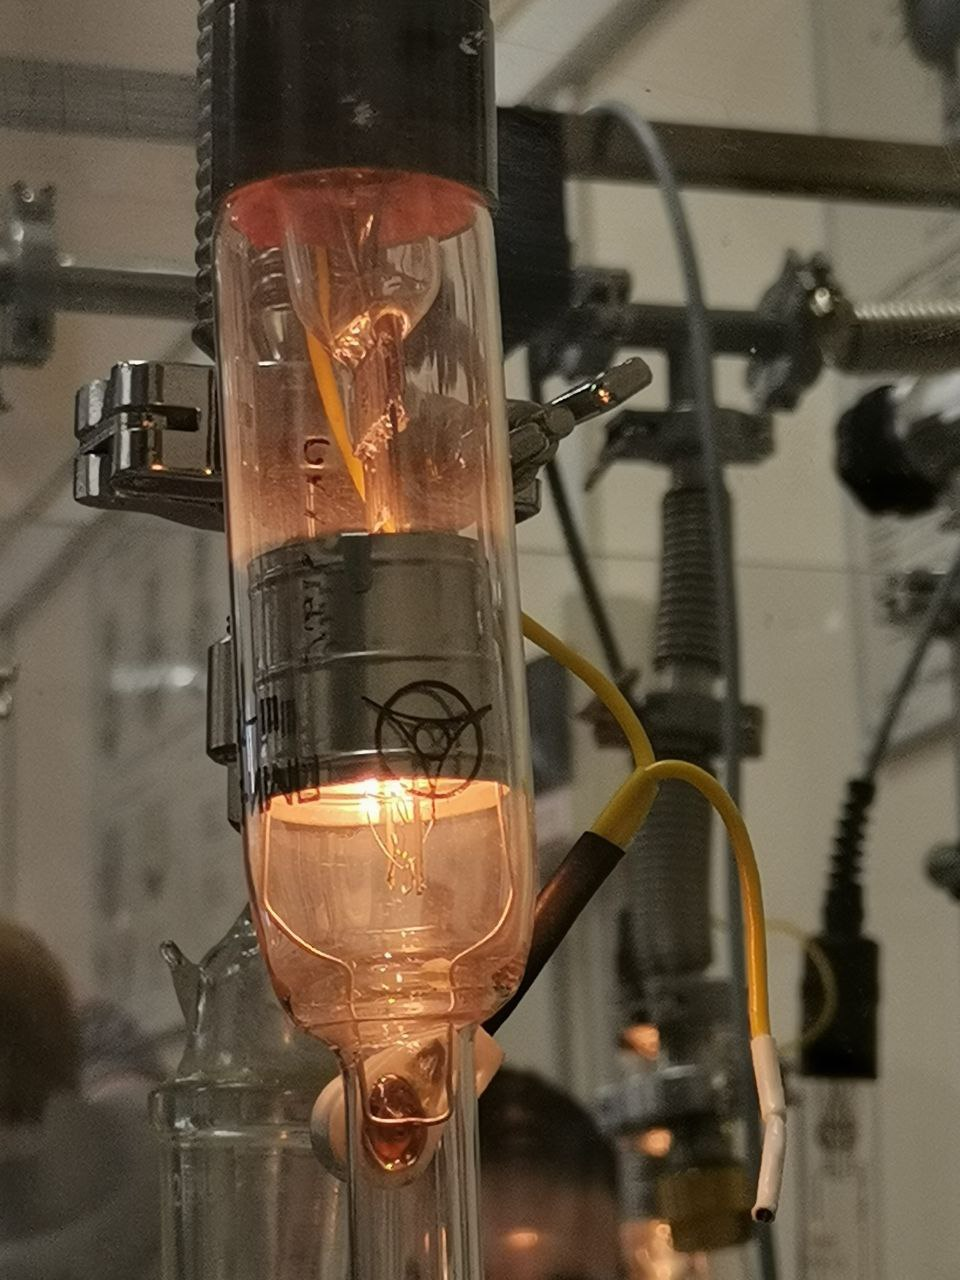
\includegraphics[scale = 0.12]{images/ion.jpg}
    \end{figure}
\end{frame}
\begin{frame}{Измерение скорости откачки газа}
   Основное уравнение откачки газа из высоковакуумного баллона:
   \[-V_hdp = (pW - Q_v - Q_c)dt\]
   при достижении \(p_{lim}\) \(\frac{dp}{dt} = 0\), тогда
   \[p_{lim}W = Q_v + Q_c\]
   проинтегрировав первое выражение получим
   \[p-p_{lim} = p_0-p_{lim}\cdot exp(-\frac{W}{V_h}t)\]
\end{frame}

\begin{frame}{Графики откачки}

\begin{minipage}{.3\textwidth}
    \small Измеряем \(p_\) Открываем кран и с помощью ионизационного манометра получаем зависимость p(t).
    Давление убывает по экспоненциальному закону:
    \[p = p_0exp(-\frac{W}{V_h}t),\]
    откуда \(W = -k_1V_h\) %\(k_1\) - коэффициэнт наклона графика 1
\end{minipage}%
\begin{minipage}{.5\textwidth}
\begin{figure}
    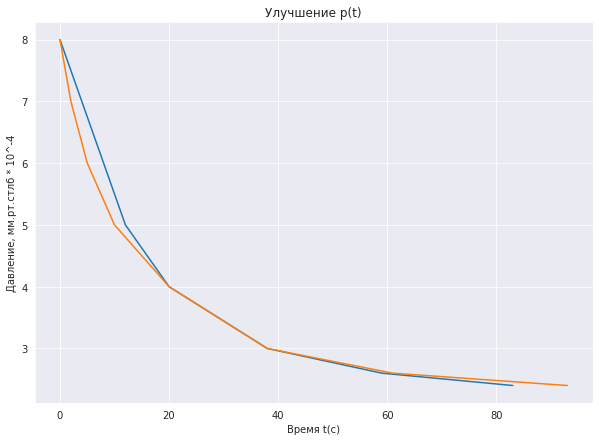
\includegraphics[scale=0.4]{images/output(decrease).png}
    \caption{Чистые данные}
    \label{fig:my_label}
\end{figure}
\end{minipage}%

\end{frame}

\begin{frame}{График откачки - Логарифм}
\begin{minipage}{0.3\textwidth}
    k_1 = -0.013 \Rightarrow  \\
    W = 4 \cdot 10^{-5} \text{ л/с}
\end{minipage}%
\begin{minipage}{.5\textwidth}
\begin{figure}
    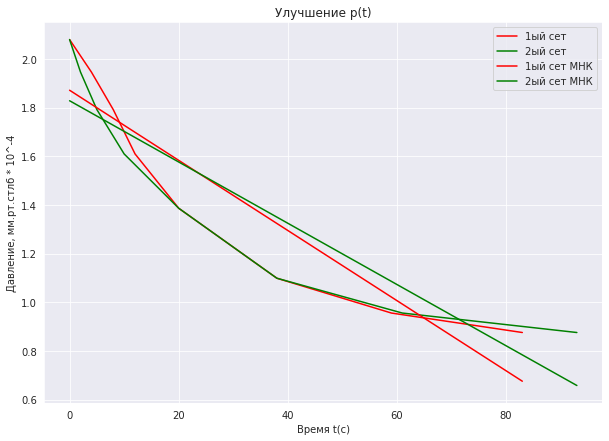
\includegraphics[scale=0.4]{images/output_decreasing.png}
    \caption{Логарифм + МНК}
    \label{fig:my_label}
\end{figure}
\end{minipage}%
\end{frame}

\begin{frame}{Графики откачки}

\begin{minipage}{.3\textwidth}
    \small Cнова закрываем кран 3 и получаем зависимость давления от времени (\(p\) от \(t\)) для истечения через микротечи, здесь насос не возвращает воздух в систему, поэтому \(Q_v = 0\) откуда:
    \[V_hdp = Q_cdt\]
    \\ $Q_c = 1.12 \cdot 10^{-4} $ 
    k_2 \text{ - коэфф. наклона} \\
    k_2 = 0.039 \Rightarrow
    Q_v = p_{lim}\cdot W - Q_c = 3.4 \cdot 10^{-4}
\end{minipage}%
\begin{minipage}{.5\textwidth}
\begin{figure}
    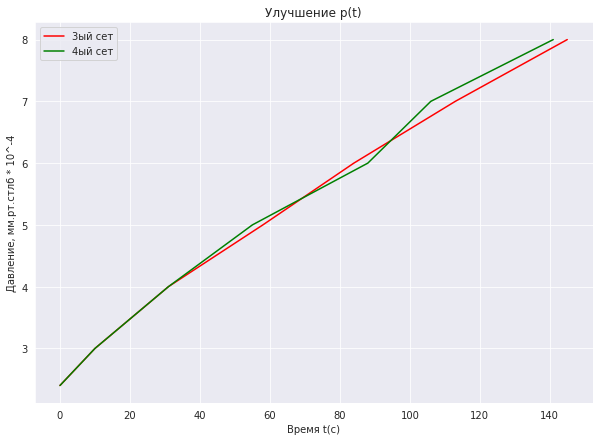
\includegraphics[scale=0.4]{images/output (decrease).png}
    \caption{Чистые данные}
    \label{fig:my_label}
\end{figure}
\end{minipage}%

\end{frame}

\begin{frame}{Вывод:}
\textbf{Вывод: } В ходе работы был получены высокий вакуум (через 3 стадии), расчитаны объемы частей насоса:
$$V_f = 1.82 \cdot 10^{-4} \text{ и } V_f = 3.1 \text{л}$$
и скорости откачки: $$Q_c = 1.12 \cdot 10^{-4} \text{ и } Q_v = 3.4 \cdot 10^{-4} \text{мВт}$$
\end{frame}

\begin{frame}{Приложение:}
    \begin{figure}
        \centering
        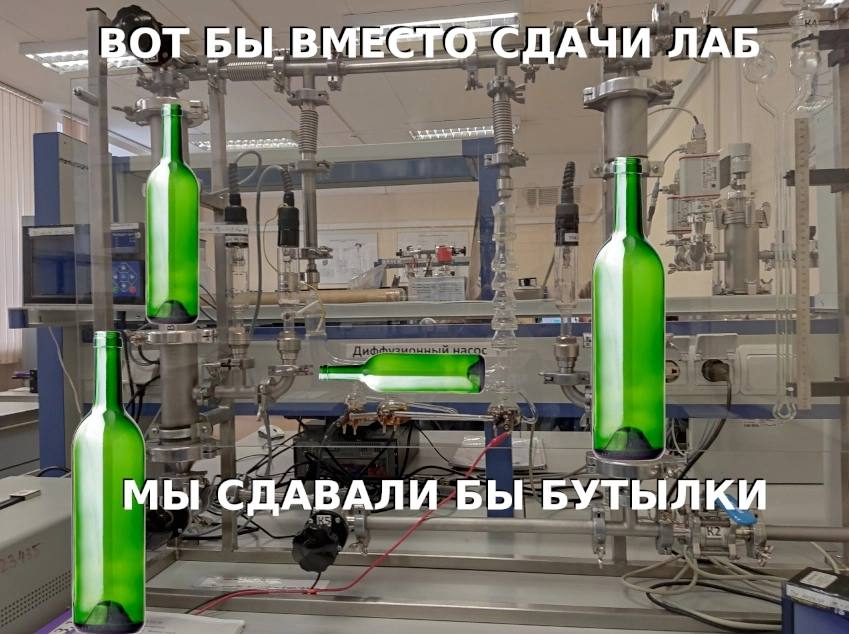
\includegraphics[scale=0.4]{images/photo_2023-02-18_00-12-39.jpg}
        \caption{Caption}
        \label{fig:my_label}
    \end{figure}
\end{frame}

\end{document}